\chapter{Metodology}
\label{chap:Metodology}

This chapter is about describing the metodology and developments to achieve the project goals. 
The python routine which this project is about was developed by the previous student that worked on it.\cite{Monica}
The software was previously developed as a electrospray multipurpose library\cite{Monica}. 


\section{Classification}
\label{sec:section_classification}

The classification is a key step in our routine. For being able to be used in multipurpose applications our classification routine must be able to run in real-time. Which means it must be fast and automatic classification.
Our goal is to improve and apply in our routine different approachs of non-visual spraying classification using the current data collected from the system.

\subsection{Statistical Analisys}

 According to Sjaaks\cite{Sjaaks}, evaluating the current data flowing through the nozzle to the plate can give us valuable information about the spraying behaviour.
 Together with the current characteristics, visual observations and results from literature it was investigated whether generic trends are present that can be related to the actual spraying modes.
 It was concluded that factors like geometry, polarity, material properties and occurring discharges are reflected in the system current.
In this work, the author also exposed some signal characteristics that can be used to classify the actual spraying mode with a sample of measured current using both time domain and frequency domain analysis.

From those analysis we are appliying in our automatic classification system the relative standard deviation. Which is refered as the sample standart deviation divided by the sample mean values.

\begin{figure}[H]
    \centering
    \resizebox{50mm}{!}{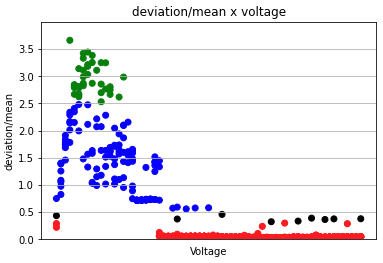
\includegraphics{Figuras/report2/data3_sjaaksgraph2.png}}
    \caption{EHDA automation system setup}
    \label{fig:sjaaks_statistical_class}
\end{figure}

 
 through statistical analysis in the signal such as mean value and standart deviation.
 Our classification by statistical analysis was implemented in the automation library made by the previous student \cite{Monica}.

 Each current sample is 0.5s of current data in 10kHz sampling frequency.
 By the processing thread we take this sample and evaluate the followings statistical values.

To classify the multijet I searched \cite{Ryan} The data thus obtained shows that in all cases the relationship between current and flow rate observed in single cone-jet mode is maintained in multi-jet mode when the current and flow rate is normalized by the number of jets. 

        
        - Sjaak Classification -> Classifies Dripping, Intermittent and Cone Jet
        
        - Monica Classification -> Classifies Corona Sparks

        - João Classification -> Classifies Multi Jet

	The algorithm implemented works in the following way:
	\begin{algorithm}
        \caption{Statistical Classification}\label{alg:statistical_class}
        \begin{algorithmic}
        \Function{statistical\_classification}{$sample$} 

            \State $spray\_mode \gets "Undefined"$;
            \State $mean \gets sample.mean$; 
            \State $std\_deviation \gets sample.std\_deviation$;
            \State $median \gets sample.median$;
            
            \If{ $mean / std\_deviation$ > 2.5}
                \Comment{Sjaak classification \cite{Sjaaks}} 
                \State $spray\_mode \gets "Dripping"$;
            \ElsIf{$ 2.5 < mean / std\_deviation < 2.5 \And mean / std\_deviation > 0.3 $}
                \State $spray\_ mode \gets "Intermittent"$;
            \ElsIf{ $mean / std\_deviation$ < 0.3}
                \State $spray\_ mode \gets "Cone Jet"$;
                \State $cone\_jet\_mean \gets mean$;
            \EndIf

            \If{ $mean / std\_deviation$ > 2.5}
                \Comment{Monica classification \cite{Monica}} 
            \EndIf

            \If{ $spray\_mode == "Cone Jet"$}
                \Comment{João classification} 
                \If{ $cone\_jet\_mean > 1.14 \times mean$}
                    \State $spray\_ mode \gets "Multi Jet"$;
                \EndIf
            \EndIf

            \Return $spray\_ mode$;
        \EndFunction
        \end{algorithmic}
    \end{algorithm}


\subsection{Machine Learning}

For the machine learning 


\section{Routine Sequences}
\label{sec:routine_sequences}

    The program developed is capable of running different types of routines. The code is also easy to implement new routines.
    Continuing the methodology, in the setup json file there is a "sequence" attribute which can be chosen between "ramp", "step", "map" or "control".
    The controller thread will manage what the algorithm must do for each sequence.
    Following our control model\ref{fig:control_model_fig}, the controller outputs are the actuators signal.
    The sampling rate is fixed to 0.5 seconds for all the experiments, and it's managed by the data\_acquisiton thread\ref{subsec:data_aquisition}.


\subsection{Ramp}



\subsection{Step}
\label{subsec:step_routine}


\begin{algorithm}
    \caption{STEP sequence in controller thread}\label{alg:stepping_algorithm}
    \begin{algorithmic}
    \Procedure{STEP}{$voltage\_start,voltage\_stop$} 
        \State $voltage \gets voltage\_start$
        \While{$voltage \leq voltage\_stop$} \Comment{scanning voltage range}
            \State \Call{send\_voltage\_command}{voltage}
            \State \Call{sleep}{step \_time}
            \State $voltage \gets voltage + step\_size$
        \EndWhile
    \EndProcedure

    \end{algorithmic}
\end{algorithm}

\subsection{Map}

The map that will be explained bellow is the most relevant sequence in this work. This type of experiment saves human work and time, create a precise analysis and can be compared with previous works for validation of methodology.
The purpose is to map the operational window, seen in Figure \ref{fig:ganan_calvo_fig}, that can be defined where the cone jet spraying mode can be stabilized based on the flow rate, voltage and the setup configuration\cite{gananCalvo}.

    \begin{figure}[H]
        \center
        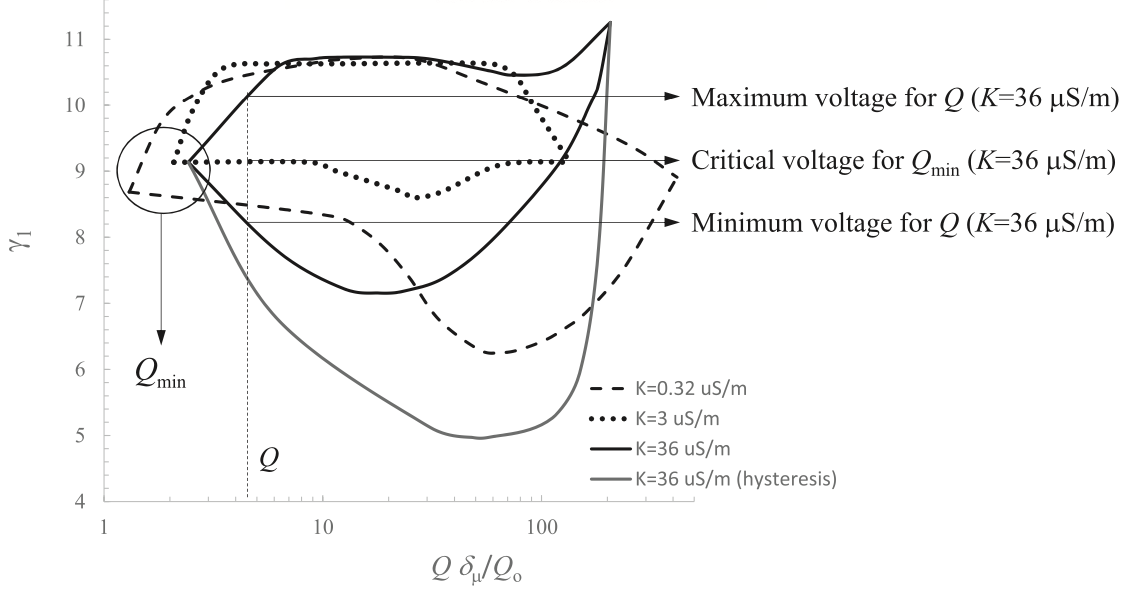
\includegraphics[width=13cm]{Figuras/ganan_calvo_map.png}
        \caption{Domains of existence (stability) of Taylor Cone Jets. \cite{gananCalvo} . The window formed by these points is where the system operated in the stable cone-jet. Operational windows depend of the liquid and configuration setup. Different windows are represented for different liquid conductivity. The X and Y axis are non-dimensional representation of electric potential and liquid flow rate, respectively.}
        \label{fig:ganan_calvo_fig}
    \end{figure}

To reach certain map it is necessary to traverse flow rate and voltage values acquiring samples.
The flow rate (X axis) and voltage (Y axis) values for each experiment can be configured in the setup.json file.
The algorithm for this sequence is a copy of the step sequence\ref{subsec:step_routine} for each flow rate chosen. It is illustrated in the algorithm \ref{alg:mapping_algorithm}.


    \begin{algorithm}
        \caption{MAP sequence in controller thread}\label{alg:mapping_algorithm}
        \begin{algorithmic}
        \Procedure{MAP}{$flowrate\_values$} 
            \ForAll{flowrate\_values}  \Comment{scanning in the flowrate range}
                \State \Call{send\_flowrate\_command}{flowrate}
                \State $voltage \gets voltage\_start$
                \While{$voltage \leq voltage\_stop$} \Comment{scanning in the voltage range}
                    \State \Call{send\_voltage\_command}{voltage}
                    \State \Call{sleep}{step \_time}
                    \State $voltage \gets voltage + step\_size$
                \EndWhile
            \EndFor
        \EndProcedure

        \end{algorithmic}
    \end{algorithm}

    In Figure \ref{fig:map2Data_fig} we can see the data acquired in this mapping experiments. The liquid used is pure ethanol. 
    Note that the experiment is composed of loops that increase voltage, change flowrate and repeat.


    \begin{figure}[H]
        \center
        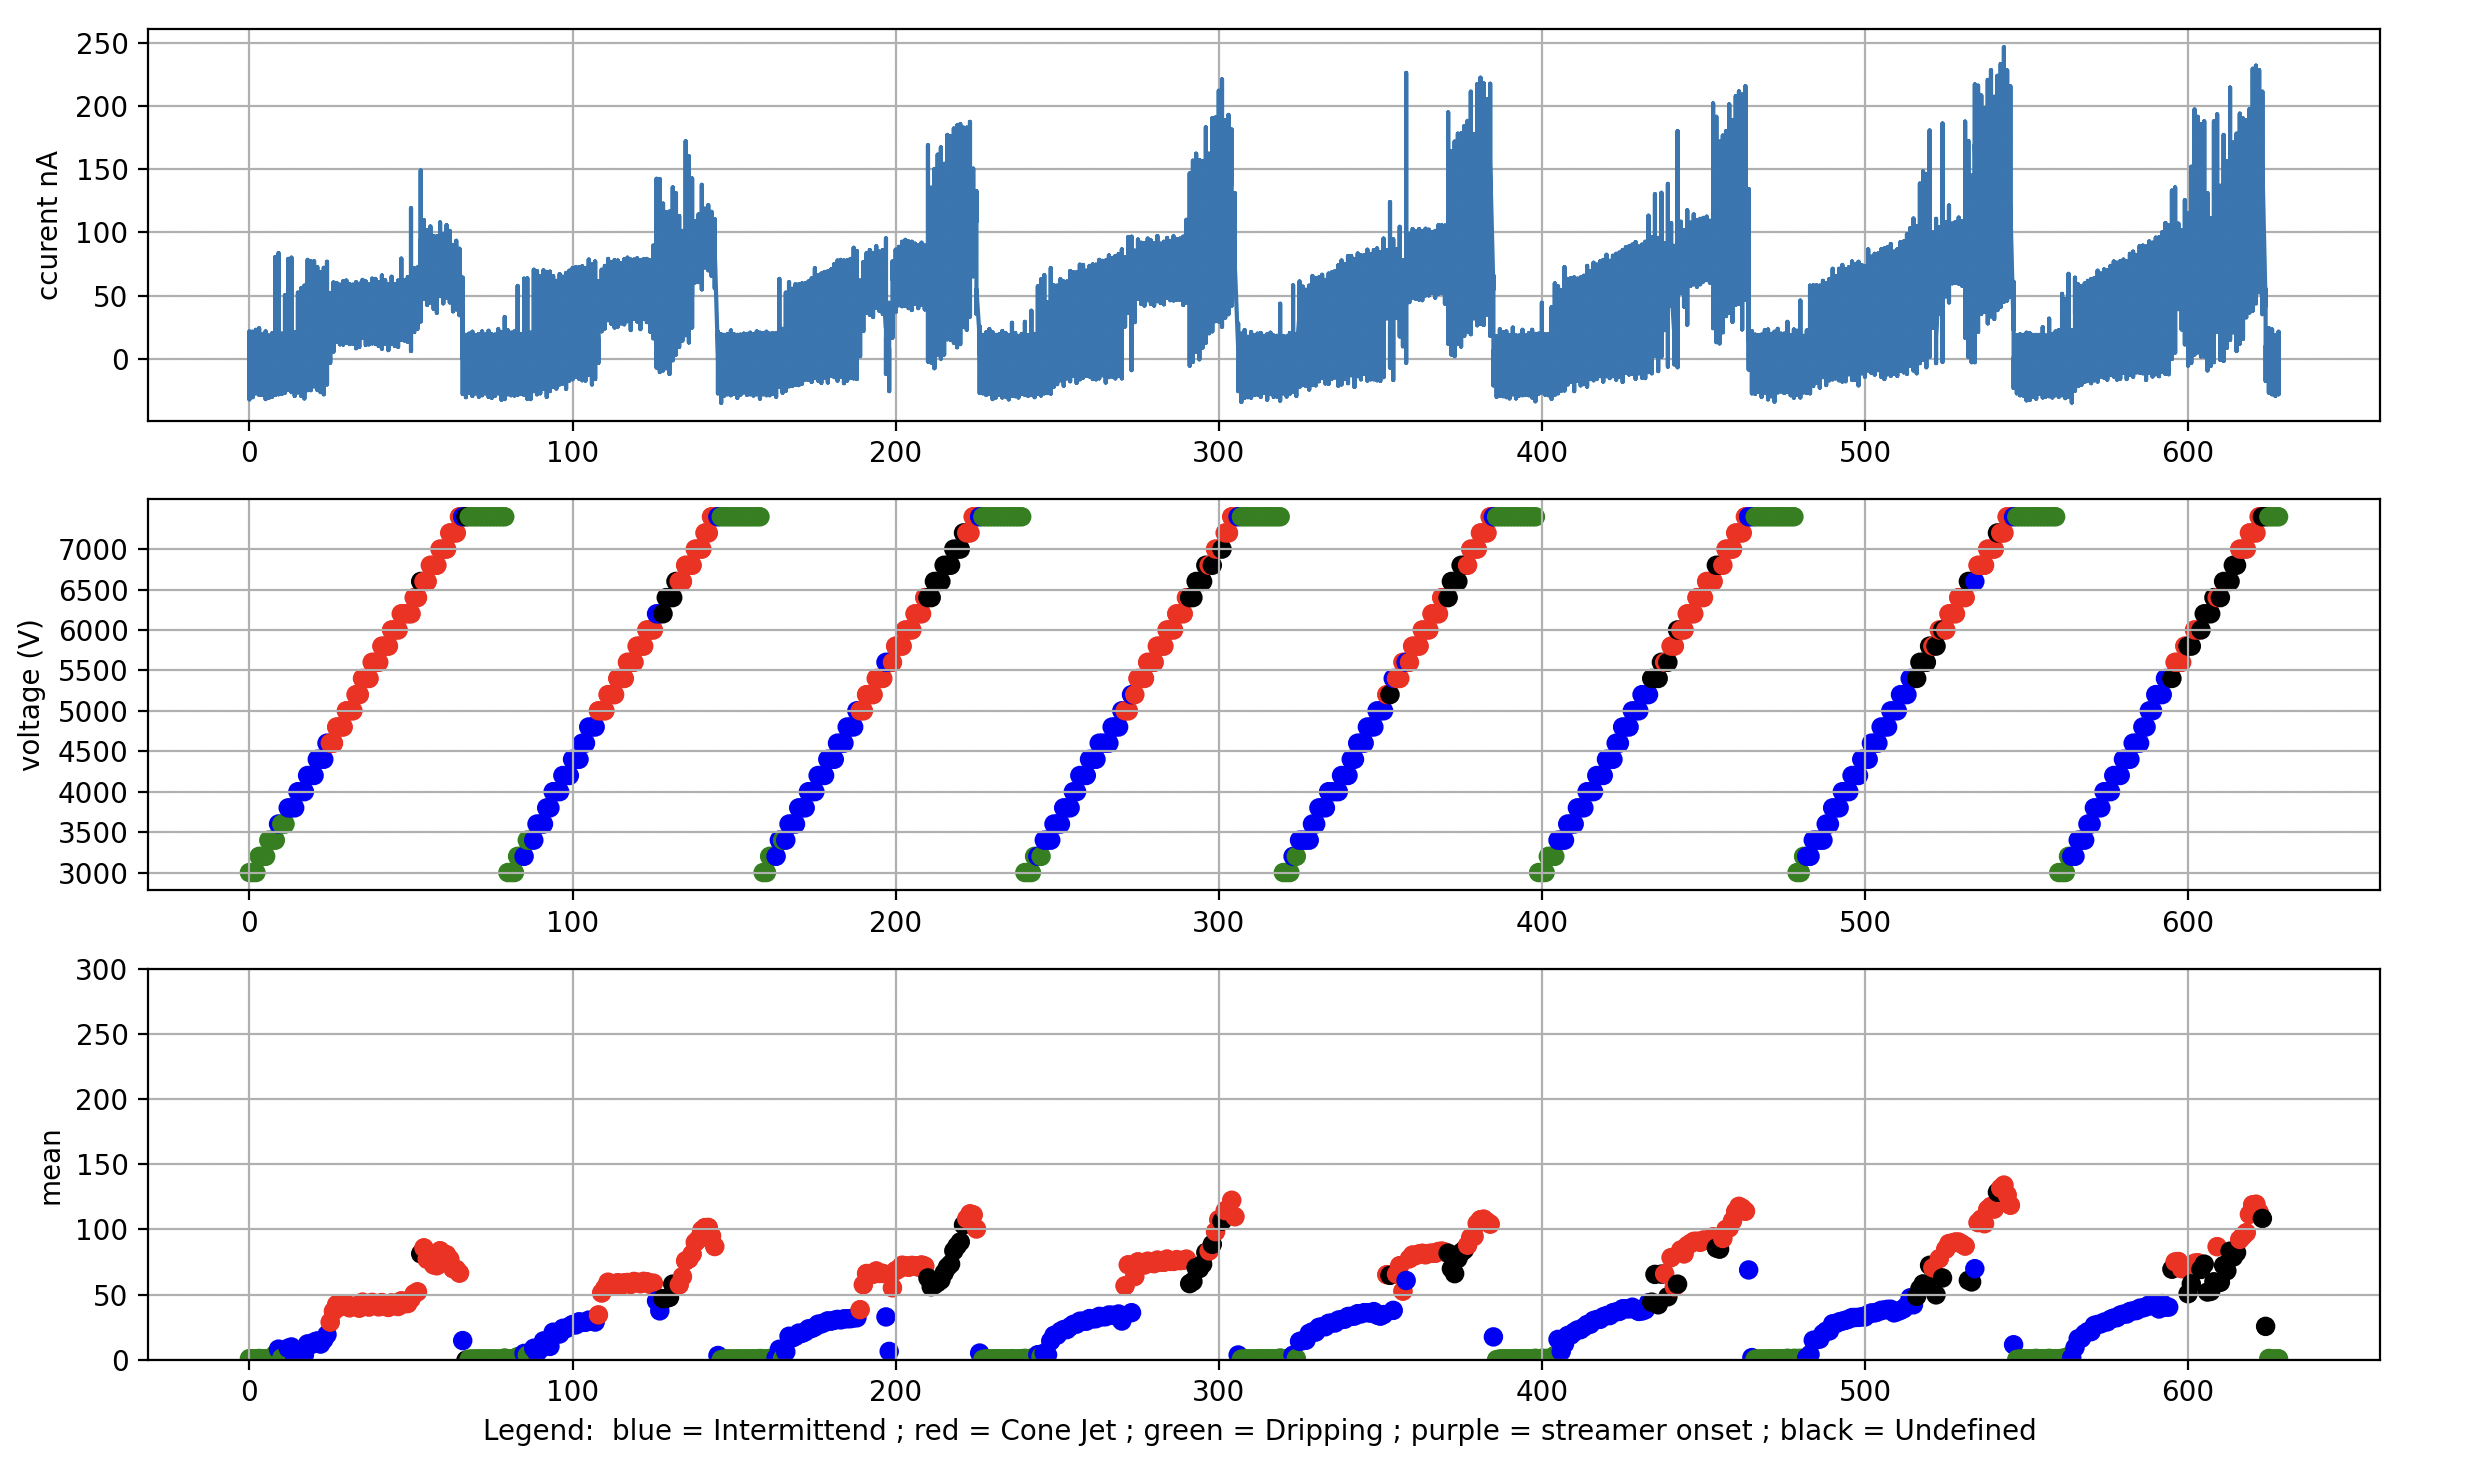
\includegraphics[width=15cm]{Figuras/report2/map2Data.png}
        \caption{Mapping Experiment data collected. The figure has 3 graphs with shared x axis representing the samples collected. The first is the current values collected through all the experiment.
        The second is the voltage values applied in each window of data collected. The colors represent the spraying classification defined by our routine.
        The third graph shows the current mean value of each data sample.}
        \label{fig:map2Data_fig}
    \end{figure}

    With all the data collected, classified and saved in real time, we can do further analysis and studies. For example, Figure \ref{fig:map3Data_fig} illustrate the data classified by our algorithm and displayed in a Voltage X FlowRate range of spraying modes with a specific liquid setup so that we can compare the automatic results with previous researchs, such as showed in figure \ref{fig:ganan_calvo_fig} and validate the algorithm.

    \begin{figure}[H]
        \center
        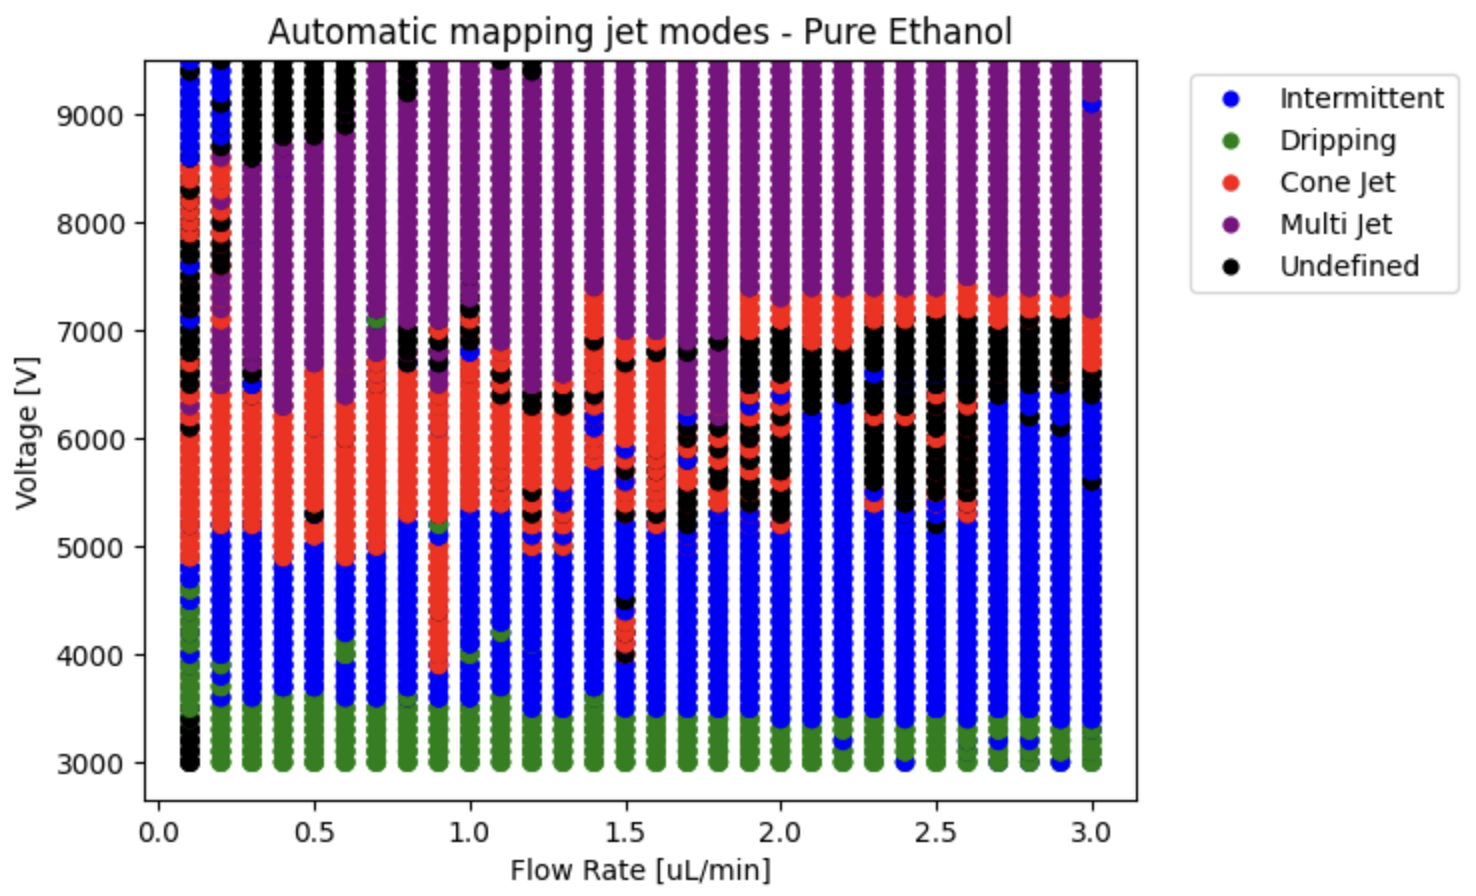
\includegraphics[width=15cm]{Figuras/report4/map-2023-03-02.png}
        \caption{Mapping Experiment for pure ethanol in ambient conditions with our capillary setup. The map shows the stability region of each electrospraying mode in the voltage and flowrate range.}
        \label{fig:map3Data_fig}
    \end{figure}



\subsection{Control}

    The control sequence is the only from our list of sequences that actually uses the feedback value. 
    As it is a closed loop control system the controller must be able to stabilize the system in the desired conditions.






\clearpage